%%%%%%%%%%%%%%%%%%%%%%%%%%%%%%%%%%%%%%%%%%%%%%%%%%%%%%%%%%%%%%%%%%%%%%%%%%
 %																		%
 %	Plantilla Latex para presentación del proyecto de curso				%
 %	Programación de Aplicaciones para Internet y la Nube					%
 %																		%
 %	Creada por: Duván Pardo, Wilson López								%
 %																		%
 %	Versión: 0.1															%
 %	Dapardoc@gmail.com ; Wilrilo@gmail.com								%
 %																		% 
 %	Se requieren los archivos plantilla.bbl y							% 
 %	El directorio Imagenes que contiene: CECAD,DC, Elementos y RITA		%  
 %																		%
%%%%%%%%%%%%%%%%%%%%%%%%%%%%%%%%%%%%%%%%%%%%%%%%%%%%%%%%%%%%%%%%%%%%%%%%%%

\documentclass[10pt]{article}   			% Describe el tipo de documento, y el tamaño de la letra del texto

\usepackage[utf8]{inputenc}				% Define codificación para que permita caracteres latinos (acentos)
\usepackage[spanish,activeacute]{babel} 	% Paquete para poder escribir con tildes y otros caracteres especiales

\usepackage{vmargin}						% Código para margenes y formato de página
\setpapersize{A4}
\setmargins	{2.2cm}     					% margen izquierdo
			{1 cm}                 		% margen superior
			{16.5cm}               		% anchura del texto
			{23.42cm}             		% altura del texto
			{20pt}                		% altura de los encabezados
			{1.2cm}               		% espacio entre el texto y los encabezados
			{0pt}                		% altura del pie de página
			{2cm}                 		% espacio entre el texto y el pie de página

\usepackage{amsmath}						% paquete para expresiones matemáticas
\usepackage{amsfonts}					% paquete para escritura de ecuaciones 
\usepackage{amssymb}						% paquete para caracteres especiales para ecuaciones 

\usepackage{fancyhdr}					% Temas para encabezado y pie de pagina
\usepackage{fancyvrb}
\pagestyle{fancy} 

\pagenumbering{arabic} 					% Numeración de paginas {arabic roman}
\usepackage{hyperref}					% Para hipervinculos
\usepackage{graphicx}					% Para incluir imágenes
\usepackage{float}	
\usepackage{caption}						% Descripciones de las figuras
\usepackage{subcaption}					% Descripción varias imagenes en usa sola figura
\graphicspath{ {Imagenes/} }				% Directorio de imágenes esta capeta va donde esta el archivo tex


\usepackage{color, colortbl}				% Colores para tablas
\usepackage{listings}					% Para el código Fuente
\usepackage{xcolor}						% para color en codigos o listrings
\definecolor{limegreen}{RGB}{50,100,50}	% Definición de colores ejemplo verde en RGB
\definecolor{Red}{RGB}{220,120,120}		% se definen colores para la tabla en el cronograma pueden ser RGB 0-255 o rgb 0-1 cada componente
\definecolor{LightCyan}{rgb}{0.88,1,1}
\definecolor{azul}{RGB}{120,120,210}


\lstset{numbers=left, numberstyle=\tiny, stepnumber=2, numbersep=5pt}

%Aquí inicia el documento.
\begin{document}
	% Se define el Encabezado
	%clhead[]{Proyecto}
	\lhead[]{Programación de Aplicaciones para Internet y la Nube}
	\rhead[]{\textbf{2016-I}}
	\renewcommand{\headrulewidth}{0.5pt}

	\thispagestyle{empty}						% La primera página no lleva estilo (sin encabezado)
	\begin{center}
		\large {Programación de Aplicaciones para Internet y la Nube
			\hspace{5 cm}\textbf{2016-I}}
		\bigskip  
		\textbf{
				\LARGE{\\TALLER 3}}\\								% Nombre del proyecto
	\end{center}	
	\begin{flushright}	
		\bigskip	
		Nombre del Estudiante: \textbf{Duván Pardo, Wilson López}			% Nombre del estudiante
	\end{flushright} 
	

\section{INTRODUCCIÓN}
Vagrant es una herramienta para crear entornos de desarrollo completos. Con un flujo de trabajo fácil de usar y centrado en la automatización, reduce el tiempo de configuración del entorno de desarrollo, aumenta la paridad entre desarrollo-producción, y hace que las "obras en mi máquina" sean una reliquia del pasado.


\textbf{Otto es el sucesor de Vagrant.}

Los creadores de Otto son también los creadores de vagrant. Después de trabajar en Vagrant más de seis años, los autores considera que Otto es una herramienta superior para el desarrollo y mucho más. Vagrant todavía llenará un papel importante para algunos usuarios, pero para la mayoría de los desarrolladores, Otto reemplazará Vagrant con el tiempo.

Aunque creen que Otto es un sucesor de Vagrant, El desarrollo de Vagrant continuará en los próximos años. Otto se basa en Vagrant, por lo que las mejoras de Vagrant beneficiarán a los usuarios Otto también. tomado de \href{https://www.vagrantup.com/about.html}{Vagran-Hashicorp} y \href{https://www.ottoproject.io/intro/vagrant-successor.html}{Otto-Hashicorp}






\section{OBJETIVO}
Realizar el despliegue de entornos de desarrollo sencillos mediante la tecnología Vagrant utilizando como proveedor de infraestructura la tecnología VirtualBox.
\section{ACTIVIDADES}	

\begin{enumerate}


	\item  Abrir una consola de comandos.
	\item Validar la correcta instalación del software Vagrant ejecutando el comando \texttt{vagrant -h}
	
	\begin{figure}[H] % Es preferible verificar la documentación para que la imagen quede correctamente segun el parámetro entre []
		\centering
		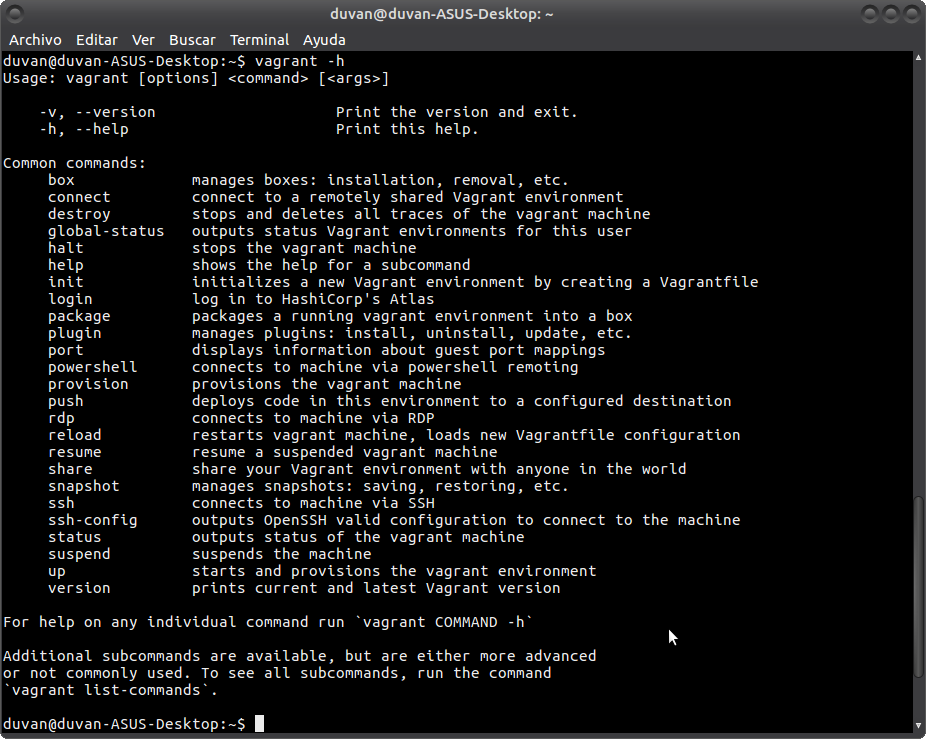
\includegraphics[scale=0.3]{2}   % Scale se utiliza para cambiar el tamaño de la imagen
		\caption{Verificación por consola de la instalación de Vagrant} 
	\end{figure}
	
	\item Adicionar la imagen del sistema operativo Ubuntu Trusty de 64 bits. Para ello, ejecutar el 	comando \texttt{vagrant box add ubuntu/trusty64} . La descarga debe tomar alrededor de 5 minutos.
	
	\begin{figure}[H] % Es preferible verificar la documentación para que la imagen quede correctamente segun el parámetro entre []
		\centering
		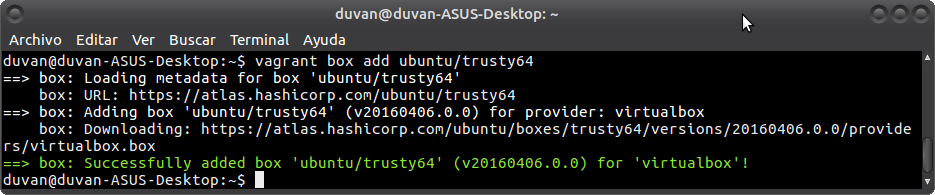
\includegraphics[scale=0.4]{3}   % Scale se utiliza para cambiar el tamaño de la imagen
		\caption{Adición del sistema operativo Ubuntu Trusty de 64 bits } 
	\end{figure}
	
	\item Crear un directorio de trabajo clouapps (o cualquier otro nombre). Ingresar a ese directorio en la consola y ejecutar el comando\texttt{ vagrant init ubuntu/trusty64}. Después de ejecutar el comando, verificar que se haya creado un archivo denominado \texttt{Vagrantfile}.
	
		\begin{figure}[ht] 
			\centering
			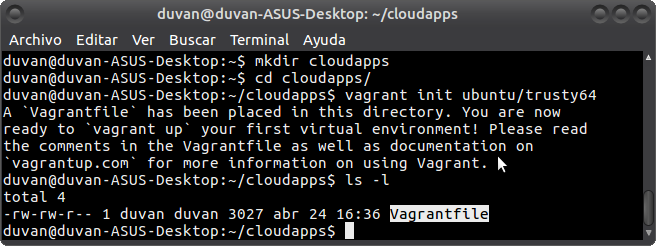
\includegraphics[scale=0.4]{4}   
			\caption{Creación del directorio clouapps} 
		\end{figure}
	
	\item Editar el archivo \texttt{\href{https://github.com/wilrilo/talleres/blob/master/file/taller3/Vagrantfile}{Vagrantfile}} de forma que contenga la siguiente información
	
	\begin{small}
		\begin{lstlisting}[frame=single]	
		
	
# -*- mode: ruby -*-
# vi: set ft=ruby :
# All Vagrant configuration is done below. The "2" in Vagrant.configure
# configures the configuration version (we support older styles for
# backwards compatibility). Please don't change it unless you know what
# you're doing.
Vagrant.configure(2) do |config|	
config.vm.box = "ubuntu/trusty64"
config.vm.network :forwarded_port, guest: 4000, host: 8100, host_ip: "127.0.0.1"
config.vm.provision "shell", path: "script.sh"
end
			
		\end{lstlisting}
	\end{small}
	
	
			\begin{figure}[H] 
				\centering
				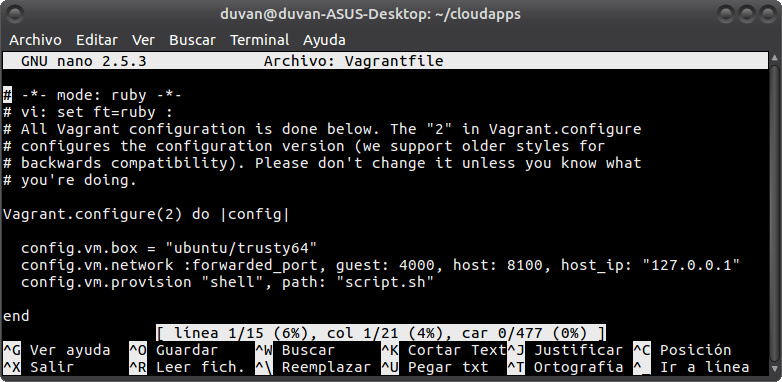
\includegraphics[scale=0.28]{5}   
				\caption{Archivo \texttt{Vagrantfile} editado.} 
			\end{figure}
			
\item Crear un archivo “\texttt{\href{https://github.com/wilrilo/talleres/blob/master/file/taller3/script.sh}{script.sh}}”  en el mismo directorio del archivo \texttt{Vagrantfile}.

\item Escribir el siguiente contenido en el archivo “\texttt{\href{https://github.com/wilrilo/talleres/blob/master/file/taller3/script.sh}{script.sh}}”
			
	
	
	\begin{small}
		\begin{lstlisting}[frame=single]	
		
#!/usr/bin/env bash	
echo &quot;Installing: nodejs, lynx, ruby and jekyll...&quot;
apt-add- repository ppa:brightbox/ruby-ng &gt;&gt;/tmp/provision-script.log ... 
2&gt;&amp;1
apt-get -y update &gt;&gt;/tmp/provision-script.log 2&gt;&amp;1
apt-get install -y nodejs &gt;&gt;/tmp/provision-script.log 2&gt;&amp;1
apt-get install -y lynx-cur &gt;&gt;/tmp/provision-script.log 2&gt;&amp;1
apt-get install -y ruby2.2 &gt;&gt;/tmp/provision-script.log 2&gt;&amp;1
apt-get install -y ruby2.2-dev &gt;&gt;/tmp/provision-script.log 2&gt;&amp;1
gem install jekyll &gt;&gt;/tmp/provision-script.log 2&gt;&amp;1
cd /vagrant
jekyll serve -H 0.0.0.0 - detach
		
		\end{lstlisting}
	\end{small}

			\begin{figure}[H] 
				\centering
				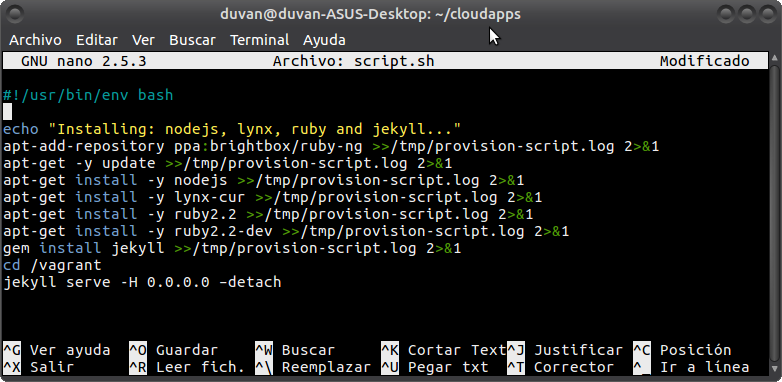
\includegraphics[scale=0.4]{6}   
				\caption{Archivo \texttt{script.sh} editado.} 
			\end{figure}	
	
\item Ejecutar el comando \texttt{vagrant up -provision}.\\


Con lo que obtenemos la siguiente respuesta:

\begin{figure}[H] 
	\centering
	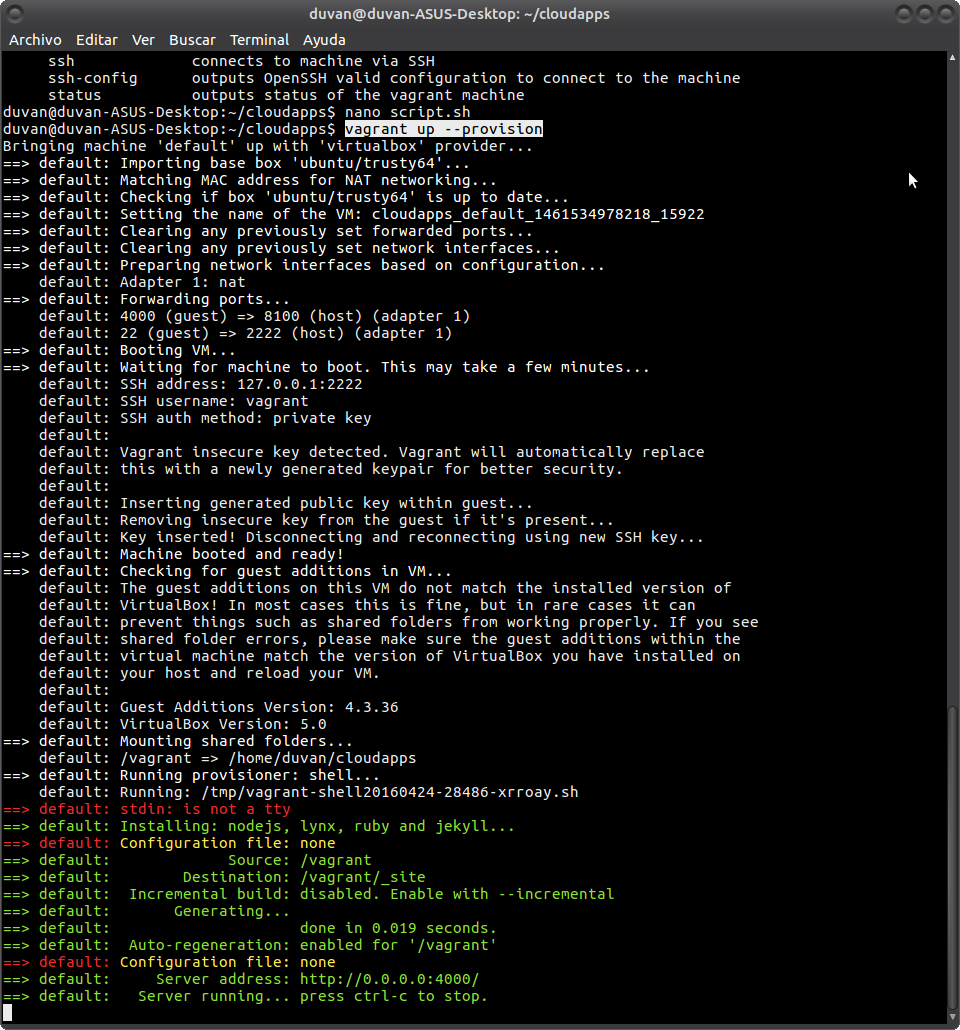
\includegraphics[scale=0.18]{8}   
	\caption{Ejecución del comando \texttt{vagrant up –provision}.} 
\end{figure}

A continuación se nuestra con mas detalle el resultado al ejecutar el comando  \texttt{vagrant up -provision}:\\
 
	
\begin{small}
	\begin{lstlisting}[frame=single]	
duvan@duvan-ASUS- Desktop:~/cloudapps$ vagrant up -- provision
Bringing machine &#39;default&#39; up with &#39;virtualbox&#39; provider...
==&gt; default: Importing base box &#39;ubuntu/trusty64&#39;...
==&gt; default: Matching MAC address for NAT networking...
==&gt; default: Checking if box &#39;ubuntu/trusty64&#39; is up to date...
==&gt; default: Setting the name of the VM: cloudapps_default_1461534978218_15922
==&gt; default: Clearing any previously set forwarded ports...
==&gt; default: Clearing any previously set network interfaces...
==&gt; default: Preparing network interfaces based on configuration...
default: Adapter 1: nat
==&gt; default: Forwarding ports...
default: 4000 (guest) =&gt; 8100 (host) (adapter 1)
default: 22 (guest) =&gt; 2222 (host) (adapter 1)
==&gt; default: Booting VM...
==&gt; default: Waiting for machine to boot. This may take a few minutes...
default: SSH address: 127.0.0.1:2222
default: SSH username: vagrant
default: SSH auth method: private key
default:
default: Vagrant insecure key detected. Vagrant will automatically replace
default: this with a newly generated keypair for better security.
default:
default: Inserting generated public key within guest...
default: Removing insecure key from the guest if it&#39;s present...
default: Key inserted! Disconnecting and reconnecting using new SSH key...
==&gt; default: Machine booted and ready!
==&gt; default: Checking for guest additions in VM...
default: The guest additions on this VM do not match the installed version of
default: VirtualBox! In most cases this is fine, but in rare cases it can
default: prevent things such as shared folders from working properly. If you see
default: shared folder errors, please make sure the guest additions within the
default: virtual machine match the version of VirtualBox you have installed on
default: your host and reload your VM.
default:
default: Guest Additions Version: 4.3.36
default: VirtualBox Version: 5.0
==&gt; default: Mounting shared folders...
default: /vagrant =&gt; /home/duvan/cloudapps
==&gt; default: Running provisioner: shell...
default: Running: /tmp/vagrant-shell20160424- 28486-xrroay.sh
==&gt; default: stdin: is not a tty
==&gt; default: Installing: nodejs, lynx, ruby and jekyll...
==&gt; default: Configuration file: none
==&gt; default: Source: /vagrant
==&gt; default: Destination: /vagrant/_site
==&gt; default: Incremental build: disabled. Enable with -- incremental
==&gt; default: Generating...
==&gt; default: done in 0.019 seconds.
==&gt; default: Auto-regeneration: enabled for &#39;/vagrant&#39;
==&gt; default: Configuration file: none
==&gt; default: Server address: http://0.0.0.0:4000/
==&gt; default: Server running... press ctrl-c to stop.

	\end{lstlisting}
\end{small}

\item  Verificar el correcto funcionamiento del despliegue accediendo en un navegador (browser) a la dirección: \\
\href{http://127.0.0.1:8100}{\texttt{http://127.0.0.1:8100}}.\\

\newpage
Se observa la correcta creación de la imagen en VirtualBox: 

\begin{figure}[ht] 
	\centering
	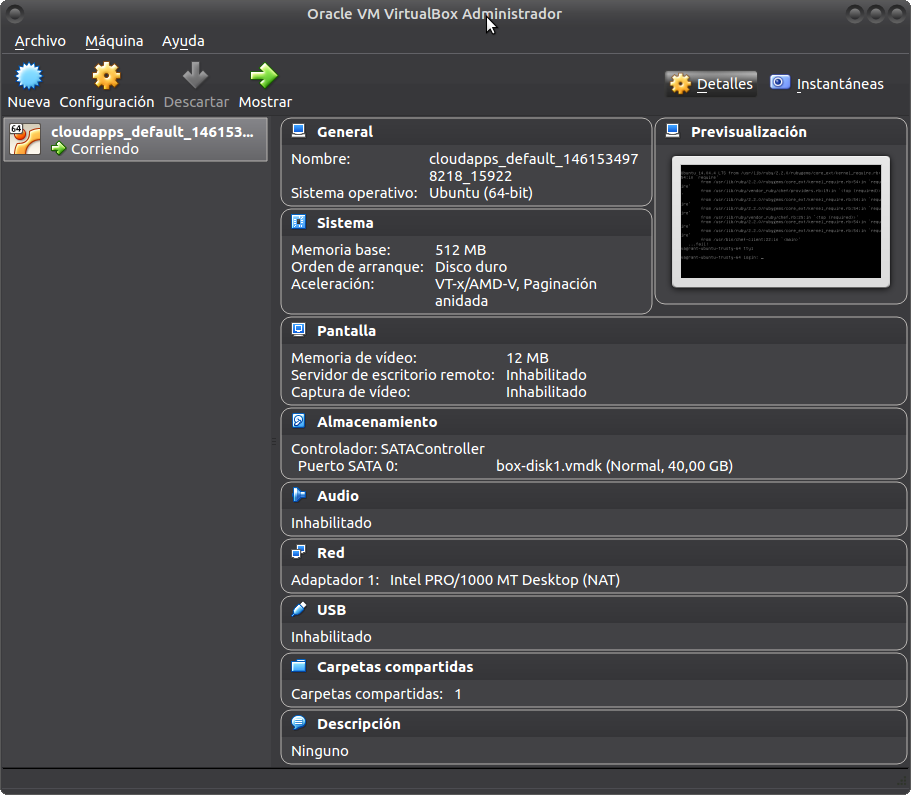
\includegraphics[scale=0.33]{VirtualBox}   
	\caption{Imagen correctamente montana en VirtualBox.} 
\end{figure}

Se procede a lanzar la maquina y verificar su funcionamiento en un navegador en la dirección: \\
\href{http://127.0.0.1:8100}{\texttt{http://127.0.0.1:8100}}.\\

\begin{figure}[ht] 
	\centering
	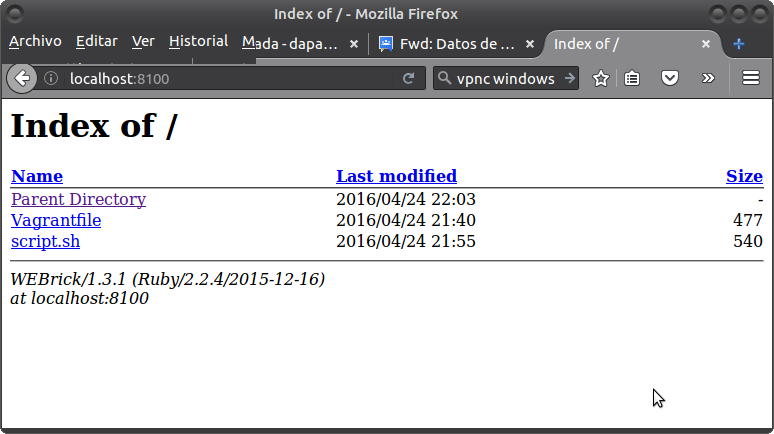
\includegraphics[scale=0.4]{9}   
	\caption{Validación del funcionamiento de la maquina virtual creada en Vagrant.} 
\end{figure}

\end{enumerate}
\section{BIBLIOGRAFÍA}
\begin{itemize}
	\item \href{https://www.vagrantup.com/about.html
		}{https://www.vagrantup.com/about.html
		}
	\item \href{https://www.ottoproject.io/intro/vagrant-successor.html	
		}{https://www.ottoproject.io/intro/vagrant-successor.html}
\end{itemize}
	
\end{document}
